\documentclass[addpoints,12pt]{exam}
\usepackage{amsmath, amssymb}
\linespread{1.1}
\usepackage{graphicx}
\usepackage{multirow}
\usepackage{moreverb}
\boxedpoints
\pointsinmargin
\usepackage[T5,T1]{fontenc}  


%\printanswers
\noprintanswers

\pagestyle{headandfoot}
\runningheadrule
\runningheader{Econ 103}
              {Final Examination, Page \thepage\ of \numpages}
              {May 9th, 2016}

\runningfooter{Name: \rule{5cm}{0.4pt}}{}{Student ID \#: \rule{5cm}{0.4pt}}


%%%%%%%%%%%%%%%%%%%%%%%%%%%%%%%%%%%%%%%%%%%%%%%%%%%%%%%%%%%%%%%
\begin{document}

\begin{center}
\large
\sc{Final Examination\\ \normalsize Econ 103, Statistics for Economists \\ \vspace{0.5em} May 9th, 2016}

\vspace{1em}

\normalsize
\fbox{\begin{minipage}{0.51\textwidth}
\textbf{\small You have 120 minutes to complete this exam.
Graphing calculators, notes, and textbooks are not permitted. }\end{minipage}}


\end{center}
%%%%%%%%%%%%%%%%%%%%%%%%%%%%%%%%%%%%%%%%%%%%%%%%%%%%%%%%%%%%%%%


\vspace{2em}
\begin{center}
  \fbox{\fbox{\parbox{5.5in}{\centering
        I pledge that, in taking and preparing for this exam, I have abided by the University of Pennsylvania's Code of Academic Integrity. I am aware that any violations of the code will result in a failing grade for this course.}}}
\end{center}
\vspace{0.2in}
\makebox[\textwidth]{Name:\enspace\hrulefill}

\vspace{0.2in}
\noindent \makebox[\textwidth]{Student ID \#:\enspace\hrulefill}

\vspace{0.3in}
\noindent\makebox[\textwidth]{Signature:\enspace\hrulefill}

%\rule{1cm}{0.4pt}
\vspace{2em}

\begin{center}
  \gradetable[h][questions]
\end{center}

\vspace{2em}

\paragraph{Instructions:} Answer all questions in the space provided, continuing on the back of the page if you run out of space. Show your work for full credit but be aware that writing down irrelevant information will not gain you points. Be sure to sign the academic integrity statement above and to write your name and student ID number on \emph{each page} in the space provided. Make sure that you have all pages of the exam before starting.

\paragraph{Warning:} If you continue writing after we call time, even if this is only to fill in your name, twenty-five points will be deducted from your final score. In addition, two points will be deducted for each page on which you do not write your name and student ID. 

%%%%%%%%%%%%%%%%%%%%%%%%%%%%%%%%%%%%%%%%%%%%%%%%%%%%%%%%%%%%%%%
\newpage
\begin{questions}

\question This question concerns the so-called ``Rademacher'' random variable, a very simple discrete RV that we did not study in Econ 103: it takes on the values $-1$ and $1$ with equal probability and never takes on any other values. 
  \begin{parts}
    \part[4] Suppose $X \sim$ Rademacher. Calculate $E[X]$
    \begin{solution}[1.5in]
     $E[X] = 1/2 \times -1 + 1/2 \times 1 = 0$
   \end{solution}
   \part[4] Suppose $X \sim$ Rademacher. Calculate $Var[X]$
   \begin{solution}[1.5in]
     $Var(X) = E[X^2] - E[X] = \left[ \left( -1 \right)^2 \times 1/2 + \left( 1 \right)^2 \times 1/2 \right]- 0 = 1$
   \end{solution}
   \part[6] Write out the CDF of the Rademacher RV.
   \begin{solution}[1.5in]
    $$F(x_0) = \left\{
    \begin{array}{ll}
      0, & x_0 < -1 \\
      1/2, & -1 \leq x_0 < 1 \\
      1, & x_0 \geq 1 
    \end{array}
    \right.$$ 
   \end{solution}
   \part[8] Suppose $X_1, X_2, X_3 \sim \mbox{ iid Rademacher}$ and define $Z = X_1 + X_2 + X_3$.
   Write out the support set and pmf of $Z$.
   \begin{solution}[2.25in]
     The support set is $\left\{ -3, -1, 1, 3 \right\}$.
     Since the underlying RVs are iid, each sequence of three outcomes has the same probability: $1/2 \times 1/2 \times 1/2 = 1/8$.
     There is only one way to get a sum of 3 ($1 + 1 + 1$) but there are three ways to get a sum of 1 since we get to choose where in the sequence to put the single -1. 
     Analogously there is only one way to get -3 and there are three ways to get -1.
     Thus: $p(-3) = 1/8,\; p(-1) = 3/8,\; p(1) = 3/8,\; p(3) = 1/8$.
   \end{solution}
   \part[10] Write an R function called \texttt{rrad} that makes iid Rademacher draws.
It should take a single argument \texttt{n} the number of iid draws and return a vector of simulations.
\begin{solution}[2.25in]
  \begin{verbatim}
rrad <- function(n){
  sample(c(-1, 1), n, replace = TRUE)
}
  \end{verbatim}
\end{solution}
\part[10] Using the function \texttt{rrad} that you constructed in the preceding part, write R code that uses 10000 simulation replications to approximate the probability that the sum of 100 iid Rademacher draws will be larger than 10. 
\begin{solution}[2.25in]
  \begin{verbatim}
sims <- replicate(10000, sum(rrad(100)))
sum(sims > 10) / length(sims)
  \end{verbatim}
\end{solution}
\part[8] Use the Central Limit Theorem to calculate the approximate value of the probability that you wrote simulation code to approximate in the preceding part.
\begin{solution}[2.5in]
  Under random sampling $\bar{X} \approx N(\mu, \sigma^2/n)$ in large samples by the Central Limit Theorem, where $\mu = E[X_i]$ and $\sigma^2 = Var(X_i)$.
  Thus, in the present example, $\bar{X} \approx N(0, 1/100)$ or equivalently $10 \bar{X} \approx N(0,1)$.
  Finally $P(X_1 + \cdots + X_{100} > 10) = P\left( \left[ X_1 + \cdots + X_{100} \right]/10 > 1 \right) = P(10 \bar{X} > 1) \approx 0.16$.
  (Note that this is slightly higher than the value of around 0.135 that you will get in R if you run the code from the previous answer: the CLT is approximate.)
\end{solution}
  \end{parts}

\question Answer each of the following: show your work or explain briefly, as applicable.
\begin{parts}
  \part[5] Let $Y \sim N(\mu = -2, \sigma^2 = 25)$.
  Approximately what is $P(Y > 8)$?
  \begin{solution}[1in]
    $P(Y > 8) = P\left[ (Y - -2)/5 > (8 - - 2)/5 \right] = P(Z > 2)$ where $Z$ is standard normal.
    Hence the probability is approximately $0.025$.
  \end{solution}
  \part[5] Let $X$ be a continuous RV with pdf $f(x)$ and support set $(-\infty, \infty)$.
  Write down the expression for $P(X > 2)$ in terms of $f$.
  \begin{solution}[1in]
    $$ P(X>2) = \int_2^{\infty} f(x) \; dx $$
  \end{solution}
  \part[5] Let $Z = X^2$ where $X \sim \mbox{N}(0,1)$.
  What kind of RV is $Z$? If it has any parameters, what values do they take? 
  \begin{solution}[1in]
    Since it equals the square of a standard normal $Z^2 \sim \chi^2(1)$.
  \end{solution}
  \part[5] The Exponential$(\lambda)$ random variable is a continuous RV that we did not study in class.
  It has one parameter, $\lambda > 0$, its support set is $[0, \infty)$ and its CDF is given by $F(x) = 1 - e^{-\lambda x}$.
    Calculate the pdf of this RV.
    \begin{solution}[1in]
      Differentiating with respect to $x$, $f(x) = F'(x) =  \lambda e^{-\lambda x}$. 
    \end{solution}
    \part[10] Use the Shortcut Rule to prove that $Cov(X, aY) = a Cov(X,Y)$ for any RVs $X,Y$ and any constant $a$.
    \begin{solution}[2in]
    By the linearity of expectation:
    \begin{eqnarray*}
      Cov(X, aY) &=& E(X \cdot aY) - E(X) E(aY)\\
      &=& a E(XY) - a E(X)E(Y)\\
      &=& a \left[ E(XY) - E(X)E(Y) \right]\\
      &=& a Cov(X,Y)
    \end{eqnarray*}
  \end{solution}
\end{parts}



\question[30] Suppose we have two independent random samples: $X_1, \hdots, X_{10} \sim \mbox{iid } N(\mu_x, \sigma_X^2 = 10)$ and $Y_1, \hdots, Y_{10} \sim \mbox{iid } N(\mu_Y, \sigma_Y^2 = 10)$
and we wish to test $H_0\colon \mu_X = \mu_Y$ against the two-sided alternative at the 5\% level. 
Derive an expression for the power of this test as a function of the true, unknown difference of population means $\Delta = \mu_X - \mu_Y$.
Your solution should involve the R command \texttt{pnorm}. 
\begin{solution}[4in]
			Since the population variances are known and both populations are normal, the test statistic
				$$T = \frac{\bar{X}_n - \bar{Y_n}}{\sqrt{\sigma_X^2/n + \sigma_Y^2/m}} = \frac{\bar{X}_n - \bar{Y}_m}{\sqrt{2}}$$
			follows a standard normal distribution under the null. This is \emph{exact} because we know the population is normal. Under the alternative $H_1\colon \mu_X \neq \mu_Y$, however, the above test statistic does \emph{not} follow a standard normal distribution. Instead,
					$$\frac{(\bar{X}_n - \bar{Y}_m) - (\mu_X - \mu_Y)}{\sqrt{2}}  \sim N(0,1)$$
					Hence, 
					$$\frac{\bar{X}_n - \bar{Y}_m}{\sqrt{2}} = \frac{(\bar{X}_n - \bar{Y}_m) - (\mu_X - \mu_Y)}{\sqrt{2}}  + \frac{\mu_X - \mu_Y}{\sqrt{2}}  \sim N\left(\frac{\mu_X - \mu_Y}{\sqrt{2}} , 1\right)$$
					In other words $T \sim N(\Delta/\sqrt{2}, 1)$. This distribution is normal, but it is only \emph{standard normal} under the null hypothesis that $\mu_X = \mu_Y$, i.e.\ $\Delta = 0$. 
		Now, at the 5\% level we reject $H_0$ when $|T| > \texttt{qnorm(1 - 0.05/2)}\approx 2$.
					Combining this decision rule with the distribution of the test statistic under the alternative, we calculate power as follows:
					\begin{eqnarray*}
						\mbox{Power}(\Delta) &=& P(\mbox{Reject } H_0|H_0 \mbox{ False})= P(|T|>2)\\
            &=& P(T < -2) + P(T > 2) \\
            &=& P(Z + \Delta/\sqrt{2} < -2) +P(Z + \Delta/\sqrt{2} > 2)\\
            &=& P(Z < -2 - \Delta/\sqrt{2}) +P(Z> 2 - \Delta/\sqrt{2})\\
            &=& \texttt{pnorm}(-2 - \Delta/\sqrt{2}) + \left[1 - \texttt{pnorm}(2 - \Delta/\sqrt{2})\right]
					\end{eqnarray*}
			\end{solution}

\question Grace polled a random sample of 800 US voters and asked them two yes or no questions:
\begin{description}
  \item[Q1 (CAR)] Do you own a car? 
  \item[Q2 (TAX)] Do you favor raising the federal gasoline tax to combat climate change? 
\end{description}
The following cross-tab contains the results of Grace's poll:
			\begin{center}
				\begin{tabular}{|cc|cc|c|}
				\hline
        &&\multicolumn{2}{c|}{\textbf{CAR}}&\\
				&&yes & no &\\
				\hline
        \multirow{2}{*}{\textbf{TAX}}
				&yes & 255 & 137 & 392\\
				&no& 350 & 58 & 408\\
        \hline
        && 605 & 195& $n=800$\\
				\hline
				\end{tabular}
			\end{center}
\begin{parts}
  \part[3] What is Grace's estimate of the fraction of US voters who favor raising the tax?
  \begin{solution}[0.75in]
    $\widehat{p} = 392/800 = 0.49$
  \end{solution}
  \part[4] Grace decides to test the null hypothesis that half of US voters favor raising the tax.
  What is the value of her test statistic? 
  Be sure to fully impose the null.
  \begin{solution}[1.5in]
    The test statistic is 
    $$\frac{\widehat{p} - 0.5}{\sqrt{0.5 \times (1 - 0.5)/n}} = \frac{0.49 - 0.5}{\sqrt{0.25/800}} \approx -0.57$$
  \end{solution}
  \part[5] Write down the R code that Grace would use to compute the two-sided p-value given for her test from the preceding part.
  \begin{solution}[0.75in]
    \texttt{2 * pnorm(-0.57)}
  \end{solution}
  \part[3] Continuing from the preceding part, would Grace reject her null hypothesis against the two-sided alternative at the 10\% significance level?
  \begin{solution}[1in]
    No: her test statistic is smaller than 1 so she wouldn't even reject the null at 32\% level.
  \end{solution}
  \part[12] Next Grace decides to test the null hypothesis that equal fractions of car-owners and non-car-owners support raising the gasoline tax.
  What is the value of her test statistic?
  Be sure to fully impose the null.
  \begin{solution}[2in]
    Of the $n = 195$ people who do not own cars, 137 support raising the tax so $\widehat{p} = 137/195 \approx 0.70$.
    In contrast, of the $m = 605$ car owners, 255 support raising the tax so $\widehat{q} = 255/605 \approx 0.42$.
    To fully impose the null in this case we need to calculate the standard error using the \emph{pooled} estimate of the population proportion: the estimate $\widehat{\pi}$ that lumps everyone together regardless of whether or not they own cars.
    Fortunately we already computed this estimate above: $\widehat{\pi} = 392/800 = 0.49$.
    The test statistic is:
    $$\frac{\widehat{p} - \widehat{q}}{\sqrt{\widehat{\pi}(1 - \widehat{\pi})\left(\displaystyle \frac{1}{n} + \frac{1}{m} \right)}} \approx \frac{0.70 - 0.42}{\sqrt{0.49 \times 0.51 \times \left( \displaystyle \frac{1}{195} + \frac{1}{605} \right)}} \approx \frac{0.28}{0.04} = 7 $$
  \end{solution}
  \part[3] Continuing from the preceding part, would Grace reject her null hypothesis against the two-sided alternative with $\alpha = 0.01$?
  \begin{solution}[1in]
    Yes: her test statistic is 7 and less than 1\% of the probability density for a standard normal random variable lies outside the range $[-3,3]$.
  \end{solution}
\end{parts}

\question This question concerns an R dataframe called \texttt{trump} that contains data for all 227 precincts in the 2016 New Hampshire Republican presidential primary.
Here are the first few rows of the data:
\begin{verbatim}
> head(trump)
        town  d_trump pvi    hhinc
1    Acworth 41.61074 Rep 57.26225
2     Albany 43.20000 Rep 58.55520
3 Alexandria 53.00546 Dem 56.25000
4 Allenstown 49.07010 Dem 54.76777
5    Alstead 45.19573 Rep 61.07143
6      Alton 42.74953 Dem 65.61787
\end{verbatim}
Each row is a precinct: \texttt{town} gives the name of the precinct, while \texttt{d\_trump} gives Donald Trump's vote share in percentage points.
The column \texttt{pvi} is a dummy variable constructed from the Cook Partisan Voter Index.
A value of \texttt{Rep} indicates that the precinct leans Republican: it voted more Republican than the US as a whole in recent presidential elections.
In contrast, a value of \texttt{Dem} indicates that the precinct leans Democratic: it voted more Democratic than the US as a whole in recent presidential elections.
Finally, \texttt{hhinc} gives the average household income in a given precinct in thousands of US dollars.
To take one particular example, consider row \#3: Donald Trump won 53\% of the vote in Alexandria, a precinct with an average household income of \$56,250 and that voted more Democratic that the US as a whole in presidential elections from the recent past.
To answer this question you will need the regression results and figures from the last two pages of this exam.
I suggest that you tear these out for easy reference.
\begin{parts}
  \part[5] Write R code to generate the boxplot comparing \texttt{hhinc} by \texttt{pvi} shown on the last page of the exam.
  You do not need to include the titles.
  \begin{solution}[1in]
\begin{verbatim}
boxplot(hhinc ~ pvi, data = trump)
\end{verbatim}
  \end{solution}
  \part[5] Briefly describe what the results of the boxplot from the preceding part suggest.
  \begin{solution}[1.5in]
    The median value of \texttt{hhinc} is higher in Democratic-leaning precincts but there is also much more variability among these precincts compared to those that lean Republican judging from the interquartile range. 
  \end{solution}
  \part[5] What is the average value of \texttt{hhinc} in Democratic-leaning precincts?
  \begin{solution}[1in]
    This is the intercept from Regression \#1: about 72.9 thousand dollars.
  \end{solution}
  \part[5] Construct an approximate 95\% confidence interval for the difference of \texttt{hhinc} between Democratic-leaning and Republican-leaning precincts. 
  \begin{solution}[1.25in]
    From Regression \#1 \texttt{hhinc} is about 7.4 thousand dollars lower on average in Republican-leaning precincts and the standard error of the difference is about 2.2 thousand dollars leading to a confidence interval of $7.4 \pm 4.4$ thousand dollars or $(\$3000, \$11,800)$. 
  \end{solution}
  \part[10] The final page of this exam shows to histograms of \texttt{hinc}: one for Democratic-leaning precincts and one for Republican-leaning precincts.
  Write R code to produce the plot for \emph{Republican-leaning precincts}.
  You do not need to include the titles
  \begin{solution}[1.25in]
\begin{verbatim}
reps <- subset(trump, pvi == "Rep")
hist(reps$hhinc)
\end{verbatim}
  \end{solution}
  \part[5] Suppose we want to predict Trump's vote share using \texttt{hhinc} \emph{only}.
  Which set of regression results should we consult?
  For two precincts that differ by \$10,000 in average household income how would we predict Trump's vote shares to differ?
  \begin{solution}[1.25in]
    Based on Regression \#3 we would predict that Trump's vote share will be 1.5 percentage points lower in the richer precinct. 
  \end{solution}
  \part[5] Continuing from the preceding part, is there a statistically significant relationship between Trump's vote share and \texttt{hhinc} at the 5\% level based on a two-sided test?
  \begin{solution}[1.25in]
    Our test statistic is $-0.15 / 0.03 = 5$ so we would very convincingly reject the null hypothesis against the two-sided alternative.
  \end{solution}
  \part[5] Where did Trump perform better: in Republican-leaning precincts or Democratic-leaining ones? 
  How much better on average?
  \begin{solution}[1.25in]
    From Regression \#5 we see that Trump performed about 5.5 percentage points \emph{worse} on average in precincts that lean Republican.
  \end{solution}
  \part[5] There are two sets of regression results that use \emph{both} \texttt{hhinc} and \texttt{pvi} to predict Trump's vote share.
  Which are they?
  Briefly explain how these two regressions differ in the way that they use the two variables to make their predictions. 
  \begin{solution}[1.5in]
    Regression \#2 allows the intercept of the relationship between \texttt{hhinc} and Trump's vote share to differ between Republican-- and Democratic--leaning precincts while Regression \#4 allows both the slope and the intercepts to differ.
  \end{solution}
  \part[6] Is there evidence of a difference in the relationship between Trump's vote share and \texttt{hhinc} in Democratic-leaning versus Republican-leaning precincts? 
  Explain briefly and justify your answer using a confidence interval.
  \begin{solution}[2in]
    Yes: from Regression \#4 the slope of the relationship between Trump's vote share and \texttt{hhinc} is 0.3 \emph{lower} in Republican-leaning precincts.
    The standard error of this difference of slopes is 0.06 leading to an approximate 95\% confidence interval of $-0.3 \pm 0.12$ or $(-0.42, -0.18)$.
    All the values in this interval are negative and large.
    We have uncovered a systematic and substantively important difference: Trump's support falls much more rapidly with income in Republican-leaning precincts.
  \end{solution}
  \part[4] Which regression most accurately predicts Trump's vote share?
  How accurate is it?
  \begin{solution}
    The most accurate is Regression \#4 which allows a different slope and intercept for the relationship between \texttt{hhinc} and Trump's vote share in Democratic-- versus Republican--leaning precincts.
    It predicts to an accuracy of about 7.2 percentage points.
  \end{solution}
\end{parts}

\newpage
\footnotesize
\paragraph{\footnotesize Regression \#1}
\begin{boxedverbatim}
lm(formula = hhinc ~ pvi, data = trump)
            coef.est coef.se
(Intercept) 72.19     1.48  
pviRep      -7.35     2.19  
---
n = 227, k = 2
residual sd = 16.45, R-Squared = 0.05
\end{boxedverbatim}
\vspace{-1em}

\paragraph{\footnotesize Regression \#2}
\begin{boxedverbatim}
lm(formula = d_trump ~ pvi + hhinc, data = trump)
            coef.est coef.se
(Intercept) 58.29     2.31  
pviRep      -6.92     1.03  
hhinc       -0.20     0.03  
---
n = 227, k = 3
residual sd = 7.56, R-Squared = 0.24
\end{boxedverbatim}
\vspace{-1em}

\paragraph{\footnotesize Regression \#3}
\begin{boxedverbatim}
lm(formula = d_trump ~ hhinc, data = trump)
            coef.est coef.se
(Intercept) 52.06     2.32  
hhinc       -0.15     0.03  
---
n = 227, k = 2
residual sd = 8.27, R-Squared = 0.09
\end{boxedverbatim}
\vspace{-1em}

\paragraph{\footnotesize Regression \#4}
\begin{boxedverbatim}
lm(formula = d_trump ~ pvi + hhinc + pvi:hhinc, data = trump)
             coef.est coef.se
(Intercept)  50.74     2.69  
pviRep       13.29     4.25  
hhinc        -0.09     0.04  
pviRep:hhinc -0.30     0.06  
---
n = 227, k = 4
residual sd = 7.20, R-Squared = 0.31
\end{boxedverbatim}
\vspace{-1em}

\paragraph{\footnotesize Regression \#5}
\begin{boxedverbatim}
lm(formula = d_trump ~ pvi, data = trump)
            coef.est coef.se
(Intercept) 44.13     0.74  
pviRep      -5.48     1.09  
---
n = 227, k = 2
residual sd = 8.21, R-Squared = 0.10
\end{boxedverbatim}

\newpage
\begin{figure}[h]
  \centering
  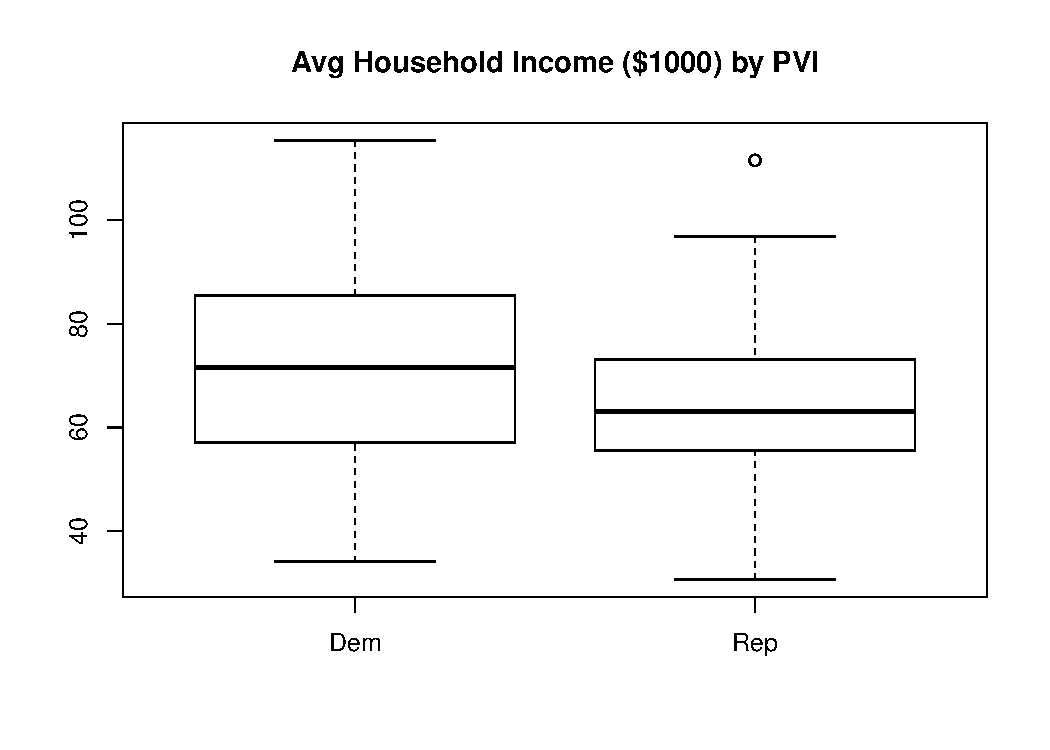
\includegraphics[scale=0.75]{final_May_2016_boxplot}\\
  \vspace{1em}
  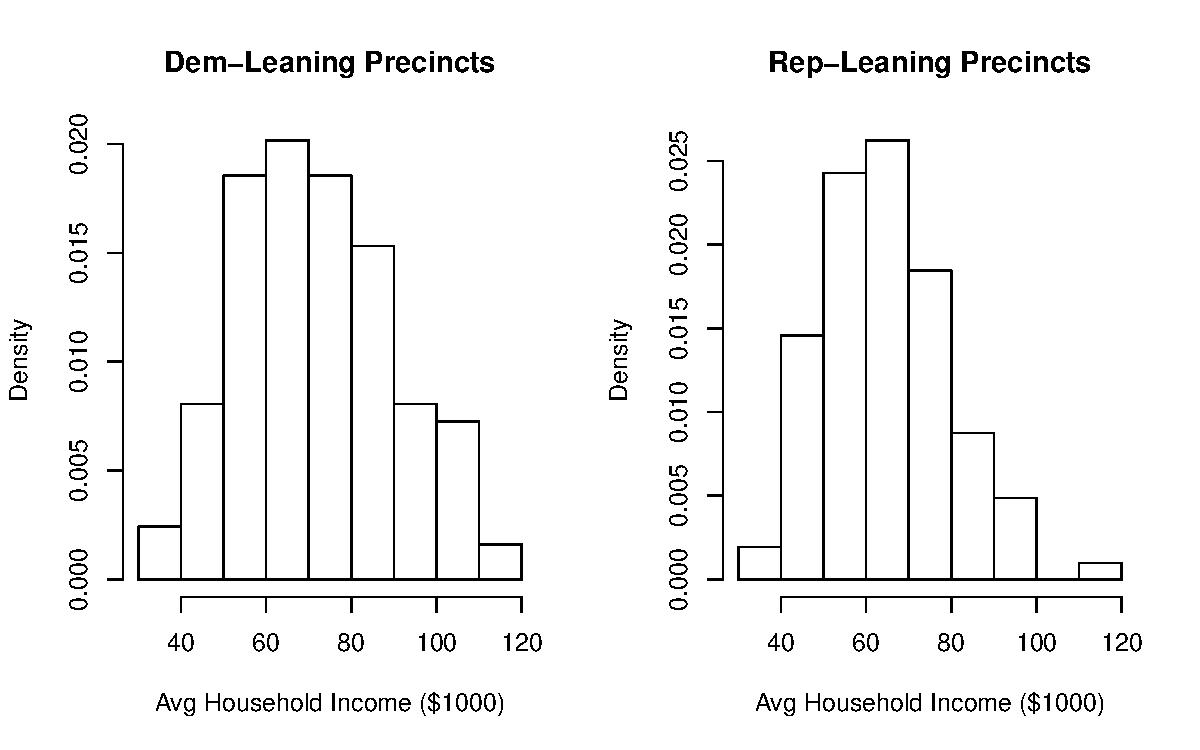
\includegraphics[scale=0.75]{final_May_2016_histograms}
\end{figure}

\end{questions}
\end{document}
